\documentclass{beamer}\usepackage[]{graphicx}\usepackage[]{color}
%% maxwidth is the original width if it is less than linewidth
%% otherwise use linewidth (to make sure the graphics do not exceed the margin)
\makeatletter
\def\maxwidth{ %
  \ifdim\Gin@nat@width>\linewidth
    \linewidth
  \else
    \Gin@nat@width
  \fi
}
\makeatother

\definecolor{fgcolor}{rgb}{0.345, 0.345, 0.345}
\newcommand{\hlnum}[1]{\textcolor[rgb]{0.686,0.059,0.569}{#1}}%
\newcommand{\hlstr}[1]{\textcolor[rgb]{0.192,0.494,0.8}{#1}}%
\newcommand{\hlcom}[1]{\textcolor[rgb]{0.678,0.584,0.686}{\textit{#1}}}%
\newcommand{\hlopt}[1]{\textcolor[rgb]{0,0,0}{#1}}%
\newcommand{\hlstd}[1]{\textcolor[rgb]{0.345,0.345,0.345}{#1}}%
\newcommand{\hlkwa}[1]{\textcolor[rgb]{0.161,0.373,0.58}{\textbf{#1}}}%
\newcommand{\hlkwb}[1]{\textcolor[rgb]{0.69,0.353,0.396}{#1}}%
\newcommand{\hlkwc}[1]{\textcolor[rgb]{0.333,0.667,0.333}{#1}}%
\newcommand{\hlkwd}[1]{\textcolor[rgb]{0.737,0.353,0.396}{\textbf{#1}}}%
\let\hlipl\hlkwb

\usepackage{framed}
\makeatletter
\newenvironment{kframe}{%
 \def\at@end@of@kframe{}%
 \ifinner\ifhmode%
  \def\at@end@of@kframe{\end{minipage}}%
  \begin{minipage}{\columnwidth}%
 \fi\fi%
 \def\FrameCommand##1{\hskip\@totalleftmargin \hskip-\fboxsep
 \colorbox{shadecolor}{##1}\hskip-\fboxsep
     % There is no \\@totalrightmargin, so:
     \hskip-\linewidth \hskip-\@totalleftmargin \hskip\columnwidth}%
 \MakeFramed {\advance\hsize-\width
   \@totalleftmargin\z@ \linewidth\hsize
   \@setminipage}}%
 {\par\unskip\endMakeFramed%
 \at@end@of@kframe}
\makeatother

\definecolor{shadecolor}{rgb}{.97, .97, .97}
\definecolor{messagecolor}{rgb}{0, 0, 0}
\definecolor{warningcolor}{rgb}{1, 0, 1}
\definecolor{errorcolor}{rgb}{1, 0, 0}
\newenvironment{knitrout}{}{} % an empty environment to be redefined in TeX

\usepackage{alltt}

\usepackage[english]{babel}
\usepackage[utf8]{inputenc}
\usepackage{multirow}

\title{Factorial Design Example: Preferences for noncontributory social policy in Latin America}

\author{ Santiago L\'opez Cariboni \\ \emph{Universidad Cat\'olica del Uruguay}~\\
Escuela de Invierno en M\'etodos y An\'alisis de Datos 2019
}

\date{}
\IfFileExists{upquote.sty}{\usepackage{upquote}}{}
\begin{document}

\begin{frame}
\maketitle


\end{frame}

\begin{frame}\frametitle{Motivation and Research question}

\begin{itemize}
	\item Non-contributory social policy have expanded in LA and increased protection among the poor. 
	\item Yet, social protection for the low-class remains being extremely narrow despite large market income inequality
	\item Insider-outsider theories suggest that labor market groups have competing preferences over social policy

\end{itemize}

Does the targeting of social policy affect social policy preferences?

\end{frame}



\begin{frame}\frametitle{Survey experiment}

Treatment 1: poor~\\
Treatment 2: informal workers~\\~\\

En este pa\'is hay muchos trabajadores [\textbf{T2: informales sin derecho al seguro de desempleo y pensiones}] que ganan un promedio de [\textbf{T1: (1/2)*Valor de linea de pobreza}] por mes. Para mejorar las condiciones de vida de esos trabajadores algunas personas apoyan que el gobierno les haga transferencias monetarias. Otros en cambio se oponen a esta medida porque incentiva el trabajo irregular o ilegal. Usted est\'a de acuerdo con realizar transferencias monetarias a estos trabajadores? ~\\



1 Muy de acuerdo 2, 3, 4, 5, 6, 7 Muy en desacuerdo.

\end{frame}
\begin{frame}\frametitle{Survey experiment}

Treatment 1: poor~\\
Treatment 2: just workers~\\~\\


En este pa\'is hay muchos trabajadores que ganan un promedio de [\textbf{T1: (1/2)*(Valor de linea de pobreza)}] por mes. Para mejorar las condiciones de vida de esos trabajadores algunas personas apoyan que el gobierno les haga transferencias monetarias. Otros en cambio se oponen a esta medida porque incentiva el trabajo irregular o ilegal. Usted est\'a de acuerdo con realizar transferencias monetarias a estos trabajadores?~\\~\\


1 Muy de acuerdo 2, 3, 4, 5, 6, 7 Muy en desacuerdo.

\end{frame}

\begin{frame}\frametitle{Survey experiment}

Treatment 1: non-poor~\\
Treatment 2: informal workers~\\~\\

En este pa\'is hay muchos trabajadores [\textbf{T2: informales sin derecho al seguro de desempleo y pensiones}] que ganan un promedio de [\textbf{T1: 2*Valor de linea de pobreza}] por mes. Para mejorar las condiciones de vida de esos trabajadores algunas personas apoyan que el gobierno les haga transferencias monetarias. Otros en cambio se oponen a esta medida porque incentiva el trabajo irregular o ilegal. Usted est\'a de acuerdo con realizar transferencias monetarias a estos trabajadores? ~\\



1 Muy de acuerdo 2, 3, 4, 5, 6, 7 Muy en desacuerdo.

\end{frame}

\begin{frame}\frametitle{Survey experiment}

Treatment 1: poor/non-poor~\\
Treatment 2: formal/informal workers~\\~\\


En este pa\'is hay muchos trabajadores que ganan un promedio de [\textbf{T1: 2*(Valor de linea de pobreza)}] por mes. Para mejorar las condiciones de vida de esos trabajadores algunas personas apoyan que el gobierno les haga transferencias monetarias. Otros en cambio se oponen a esta medida porque incentiva el trabajo irregular o ilegal. Usted est\'a de acuerdo con realizar transferencias monetarias a estos trabajadores?~\\~\\


1 Muy de acuerdo 2, 3, 4, 5, 6, 7 Muy en desacuerdo.

\end{frame}
\begin{frame}\frametitle{Survey experiment}

Treatment 1: non-poor~\\
Treatment 2: just workers~\\~\\


En este pa\'is hay muchos trabajadores que ganan un promedio de [\textbf{T1: $2 *$ (Valor de linea de pobreza)}] por mes. Para mejorar las condiciones de vida de esos trabajadores algunas personas apoyan que el gobierno les haga transferencias monetarias. Otros en cambio se oponen a esta medida porque incentiva el trabajo irregular o ilegal. Usted est\'a de acuerdo con realizar transferencias monetarias a estos trabajadores?~\\~\\


1 Muy de acuerdo 2, 3, 4, 5, 6, 7 Muy en desacuerdo.

\end{frame}





\begin{frame}\frametitle{Expected outcomes}
    
\begin{table}[tb]
	\caption{Factorial experiment; targeting to the informal and poor}
	\label{tab:tablename}
	\centering

	\begin{tabular}{ll|cc}
	\hline

	\hline

	&\textbf{} & \multicolumn{2}{c}{Informal sector} \\
	&\textbf{} & \textbf{$T_2=0$} & \textbf{ $T_2=1$} \\
	\hline
\multirow{2}{*}{Poor}	&\textbf{$T_1=0$} & E[Y$|$Z00] = 4.0   & E[Y$|$Z01] = 3.6 \\
	                    &\textbf{$T_1=1$} & E[Y$|$Z10] = 4.4   & E[Y$|$Z11] = 4.6 \\
	\hline

	\hline
	\end{tabular}
\end{table}

\end{frame}


\begin{frame}[t]\frametitle{Marginal effects}
\begin{table}[tb]
	\centering

	\begin{tabular}{ll|cc}
	\hline

	\hline

	&\textbf{} & \multicolumn{2}{c}{Informal sector} \\
	&\textbf{} & \textbf{$T_2=0$} & \textbf{ $T_2=1$} \\
	\hline
\multirow{2}{*}{Poor}	&\textbf{$T_1=0$} & E[Y$|$Z00] = 4.0   & E[Y$|$Z01] = 3.6 \\
	                    &\textbf{$T_1=1$} & E[Y$|$Z10] = 4.4   & E[Y$|$Z11] = 4.6 \\
	\hline

	\hline
	\end{tabular}
\end{table}

\begin{small}
Marginal Effect of $T_1 | T_2 = 0$: \\
$E[Y|Z10] - E[Y|Z00] = 4.4 - 4 = 0.4$ ~\\~\\

Marginal Effect of $T_1|T_2 = 1$: ~\\
$E[Y|Z11] - E[Y|Z01] = 4.6 - 3.6 = 1$~\\~\\

Marginal Effect of $T_2| T_1 = 0:$~\\
$E[Y|Z01] - E[Y|Z00] = 3.6 - 4 = -0.4$~\\~\\

Marginal Effect of $T_2|T_1 = 1$: ~\\
$E[Y|Z11] - E[Y|Z10] = 4.6 - 4.4 = 0.2$~\\~\\	
\end{small}

\end{frame}



\begin{frame}[t]\frametitle{Marginal effects}
\begin{table}[tb]
	\centering

	\begin{tabular}{ll|cc}
	\hline

	\hline

	&\textbf{} & \multicolumn{2}{c}{Informal sector} \\
	&\textbf{} & \textbf{$T_2=0$} & \textbf{ $T_2=1$} \\
	\hline
\multirow{2}{*}{Poor}	&\textbf{$T_1=0$} & E[Y$|$Z00] = 4.0   & E[Y$|$Z01] = 3.6 \\
	                    &\textbf{$T_1=1$} & E[Y$|$Z10] = 4.4   & E[Y$|$Z11] = 4.6 \\
	\hline

	\hline
	\end{tabular}
\end{table}
    
\begin{small}
Average Marginal Effect of $T_1$: ~\\
$\frac{1}{2}(E[Y|Z10] - E[Y|Z00] + E[Y|Z11] - E[Y|Z01]) = 0.5(0.4 + 1) = 0.7$~\\~\\

Average Marginal Effect of $T_2$:~\\
$\frac{1}{2}(E[Y|Z01] - E[Y|Z00] + E[Y|Z11] - E[Y|Z10])= 0.5(-0.6 + 0.2) = -0.4$~\\~\\

Conditional Marginal Effect of $T_1|T_2$ (equivalent to CME of $T_2|T_1$):~\\
$(E[Y|Z11] - E[Y|Z10]) - (E[Y|Z01] - E[Y|Z00]) = 0.2 - (-0.4) = 0.6$~\\
$(E[Y|Z11] - E[Y|Z01]) - (E[Y|Z10] - E[Y|Z00]) = 1 - 0.4 = 0.6$
\end{small}
\end{frame}


\begin{frame}\frametitle{Sample and Power}
Power analysis under \textbf{simple randomization}
    
\begin{figure}[htbp]
	\centering
\begin{table}
	\begin{tabular}{cc}
	$n=300$	& $n=400$  \\
	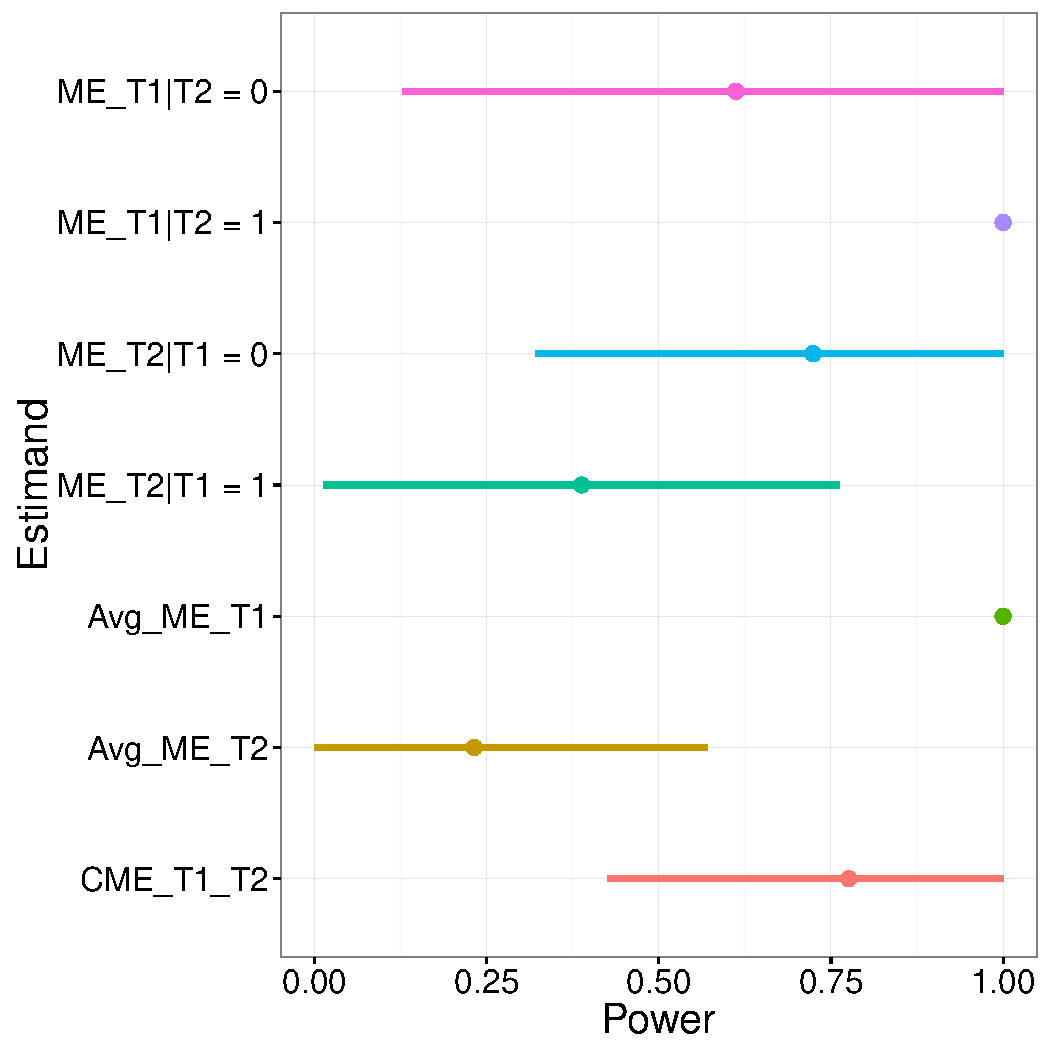
\includegraphics[width=0.45\textwidth]{power300}	& 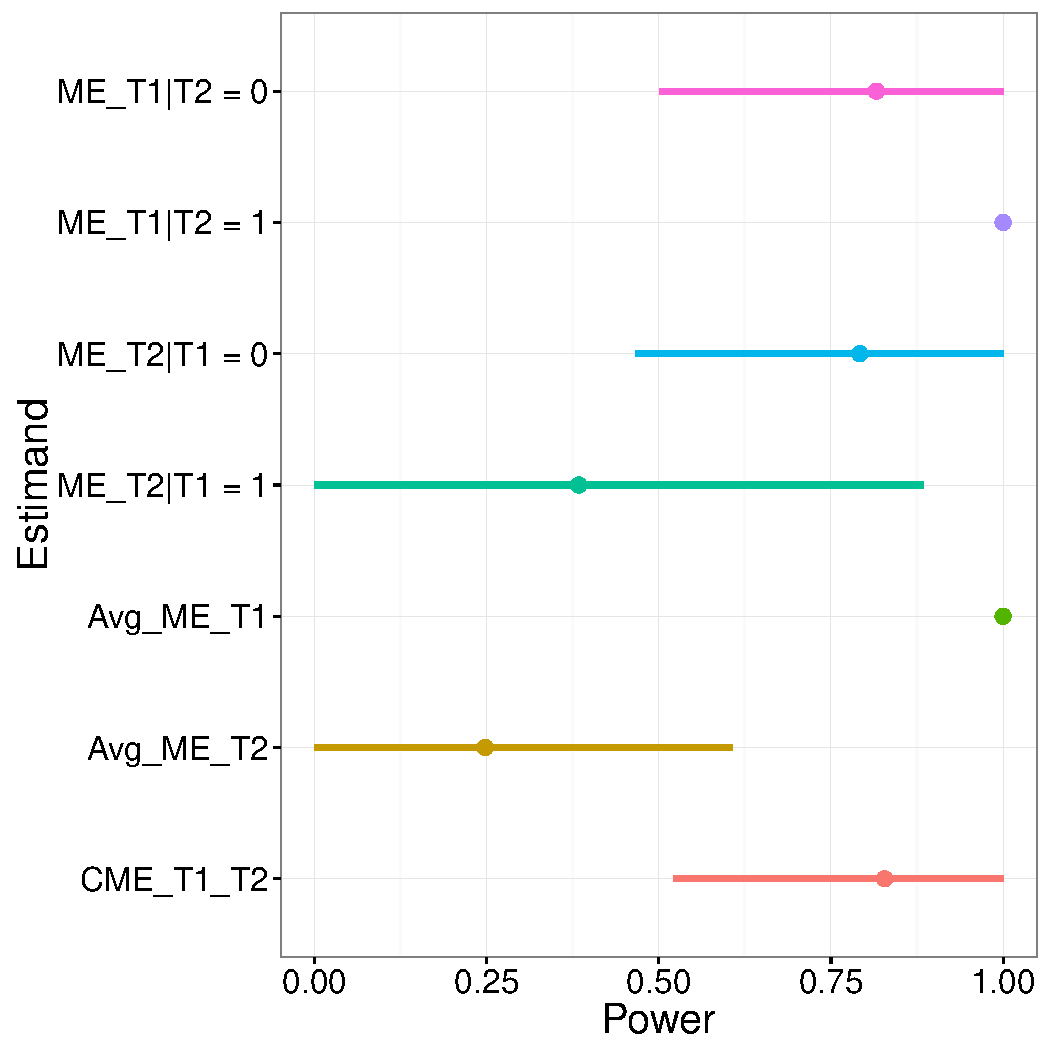
\includegraphics[width=0.45\textwidth]{power400}  \\
	\end{tabular}
\end{table}
\end{figure}
    
\end{frame}
\begin{frame}\frametitle{Sample and Power}
Power analysis under \textbf{simple randomization}
    
\begin{figure}[htbp]
	\centering
\begin{table}
	\begin{tabular}{cc}
	$n=500$	& $n=600$  \\
	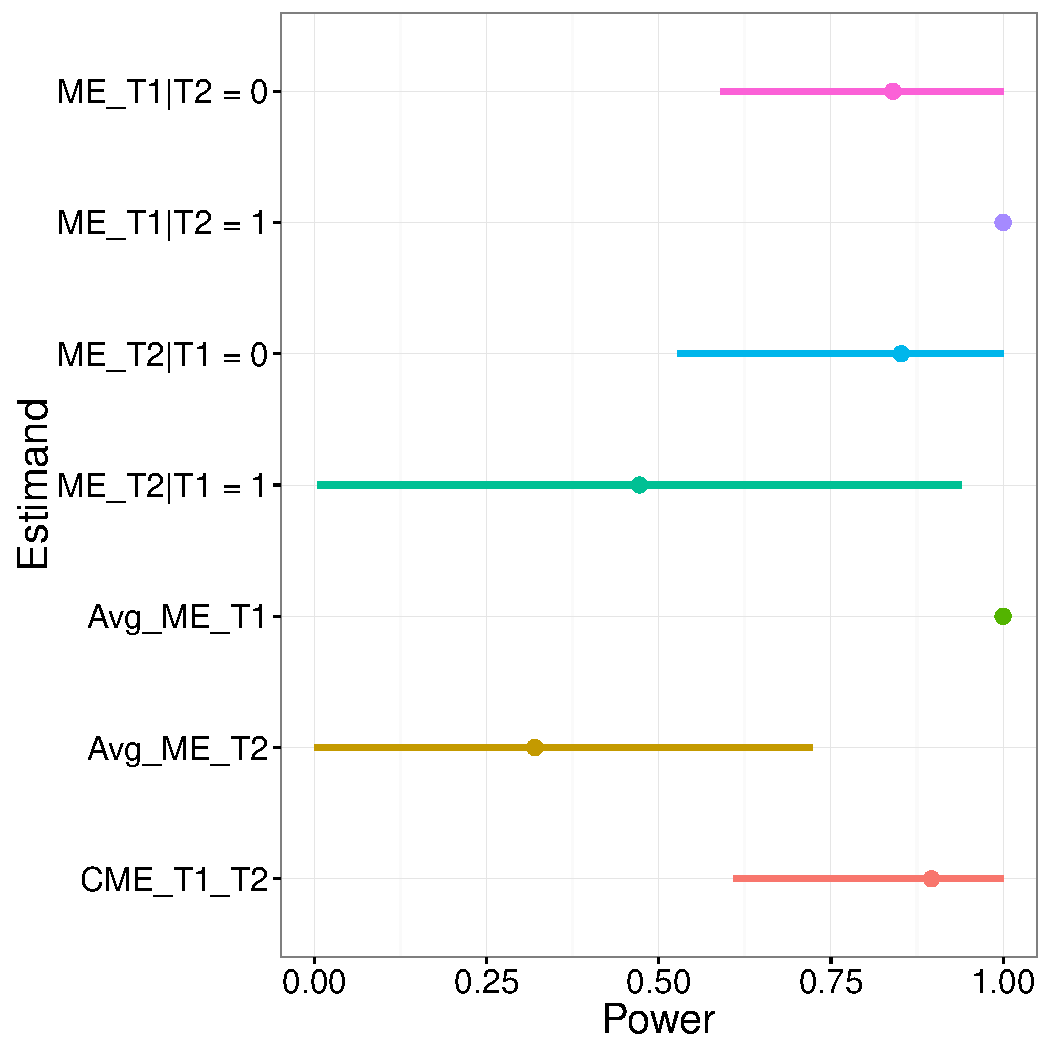
\includegraphics[width=0.45\textwidth]{power500}	& 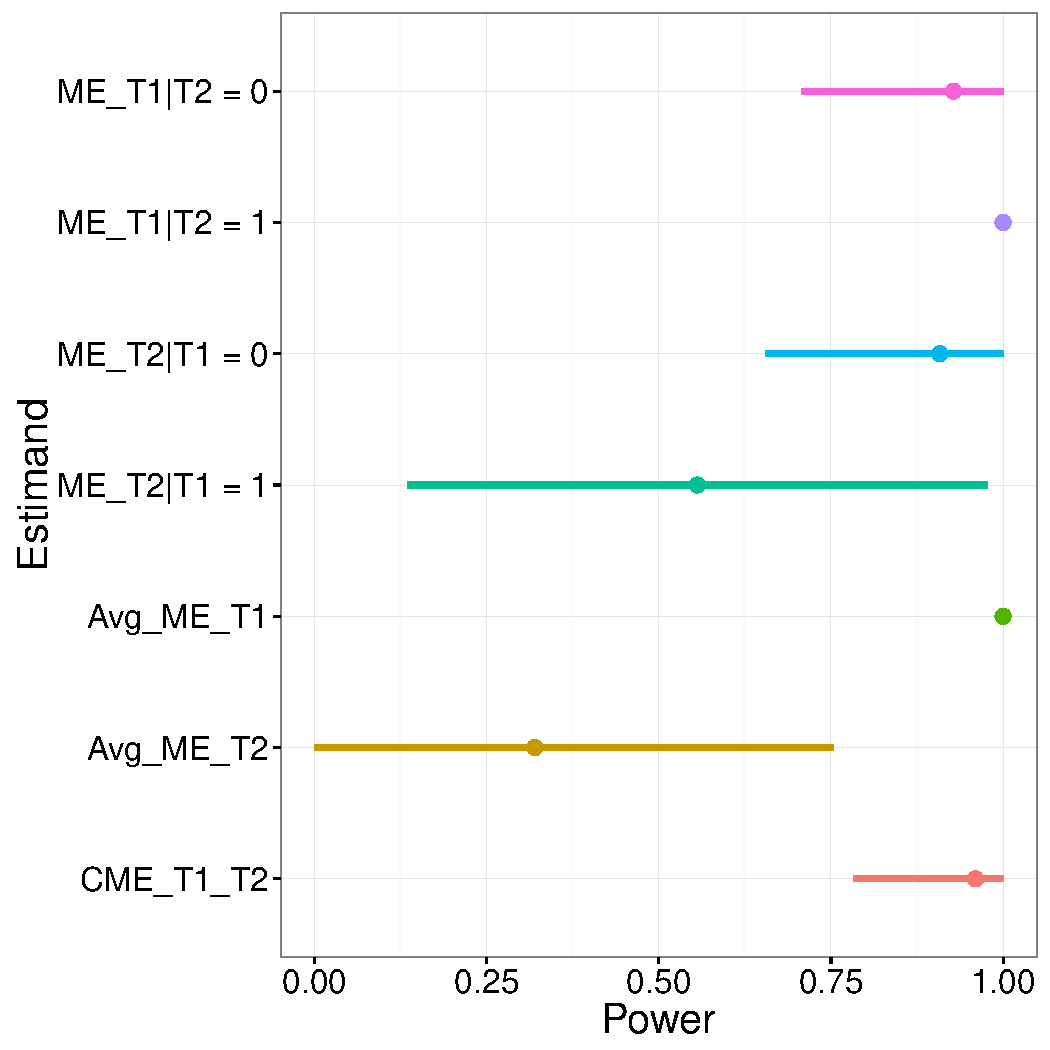
\includegraphics[width=0.45\textwidth]{power600}  \\
	\end{tabular}
\end{table}
\end{figure}
    
\end{frame}




\begin{frame}\frametitle{Sample and Power}
Power analysis under \textbf{block randomization}: income (low, middle, high) and respondent job-status (formal, informal) 
    
\begin{figure}[htbp]
	\centering
\begin{table}
	\begin{tabular}{cc}
	$n=300$	& $n=400$  \\
	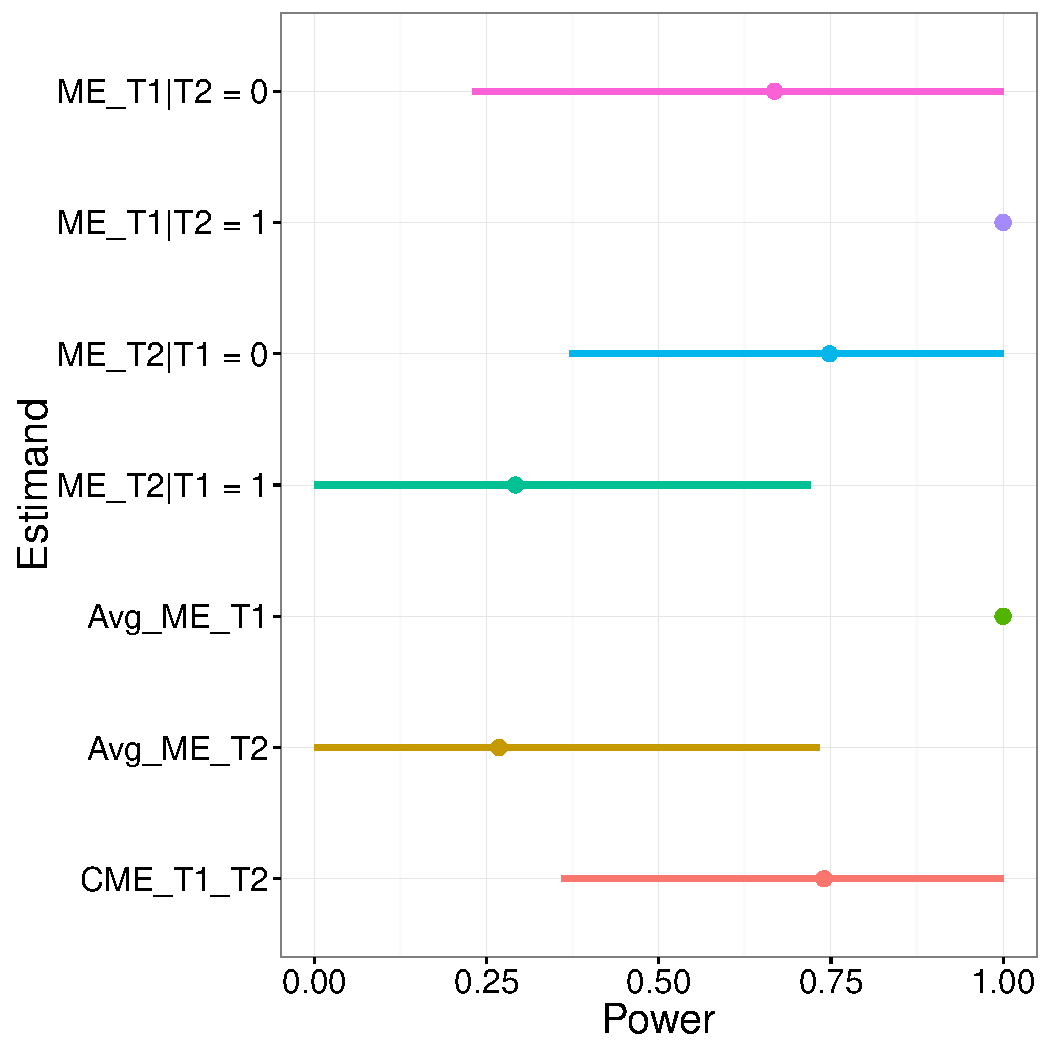
\includegraphics[width=0.45\textwidth]{power300_bra}	& 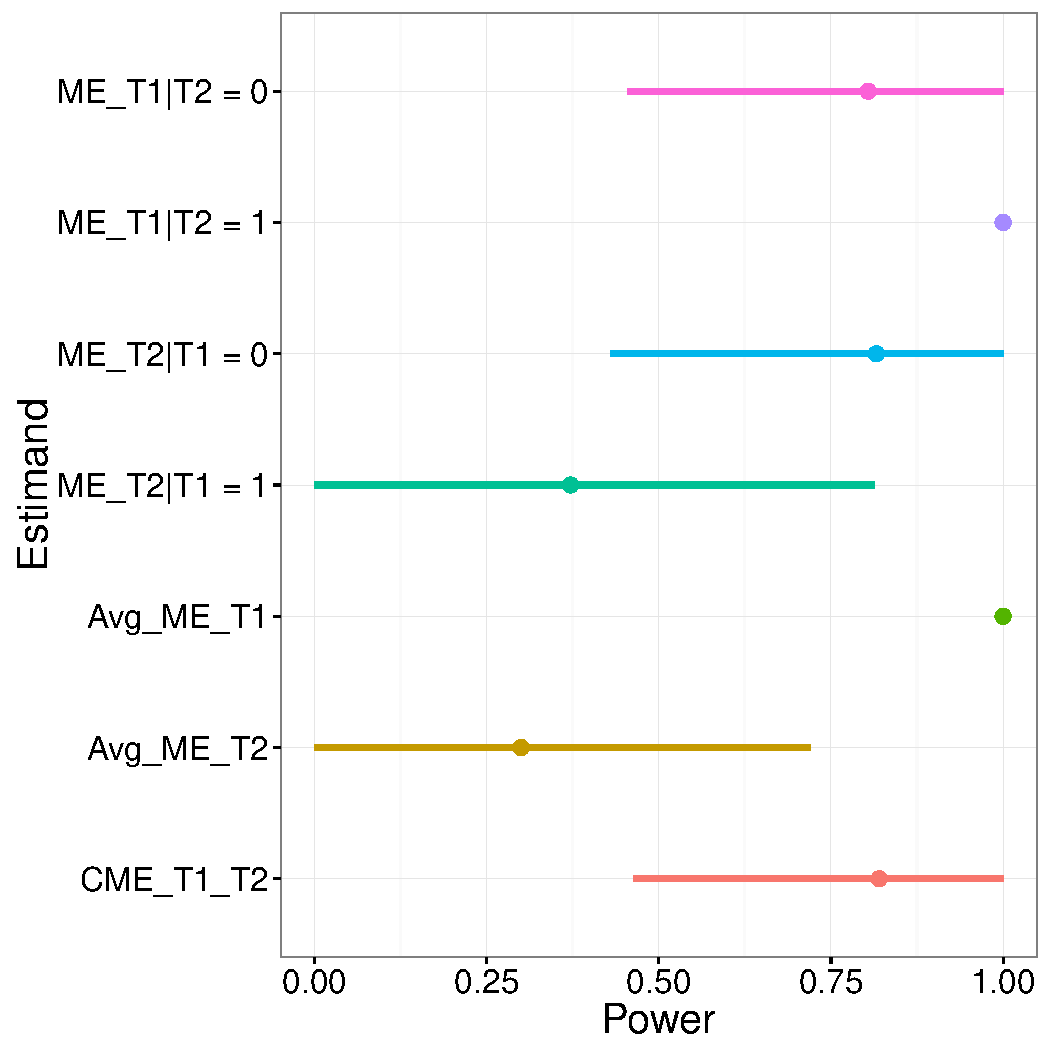
\includegraphics[width=0.45\textwidth]{power400_bra}  \\
	\end{tabular}
\end{table}
\end{figure}
    
\end{frame}
\begin{frame}\frametitle{Sample and Power}
Power analysis under \textbf{block randomization}: income (low, middle, high) and respondent job-status (formal, informal) 
    
\begin{figure}[htbp]
	\centering
\begin{table}
	\begin{tabular}{cc}
	$n=500$	& $n=600$  \\
	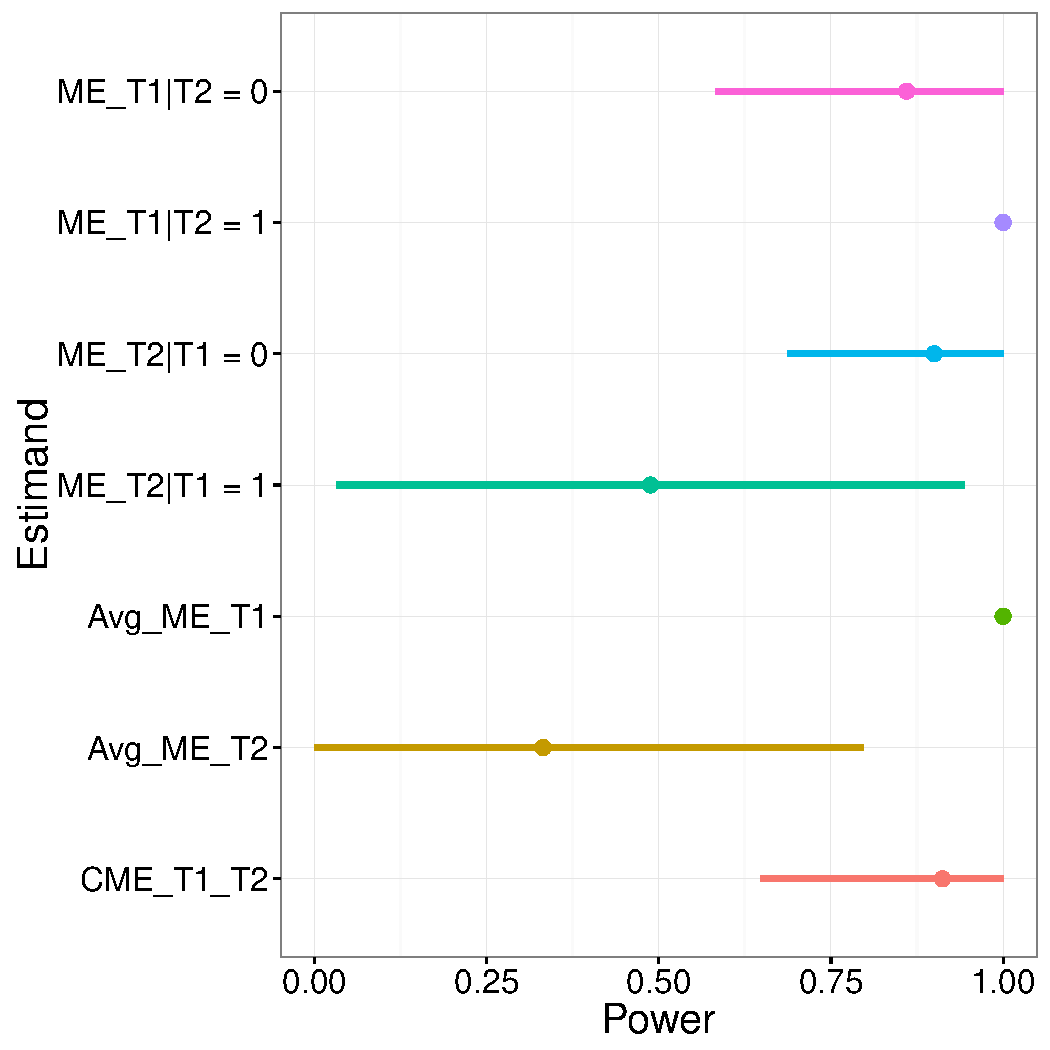
\includegraphics[width=0.45\textwidth]{power500_bra}	& 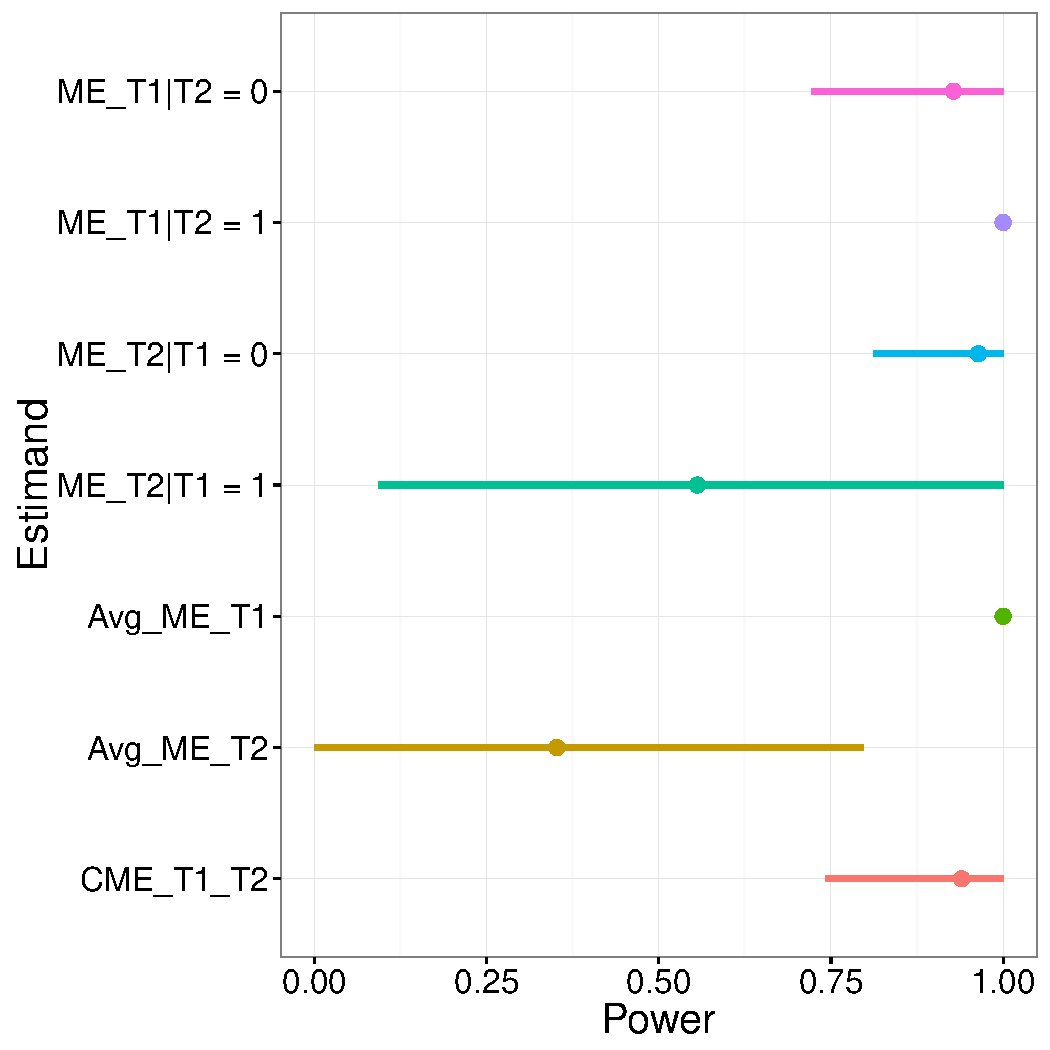
\includegraphics[width=0.45\textwidth]{power600_bra}  \\
	\end{tabular}
\end{table}
\end{figure}
    
\end{frame}



\begin{frame}\frametitle{More on Design}
    


\begin{itemize}
	\item Wording and treatments (power consumption instead of income?)
	\item Knowing more about the DV (other existing surveys)
	\item heterogeneous effects at the individual level: 
	\begin{itemize}
		\item individual perceptions of informality (``exclusion'' versus ``exit'')
		\item income
		\item job-status
		\item private social security
	\end{itemize}
	\item heterogeneous effects at the country level:
		\begin{itemize}
		 	\item labor market regulations (i.e., protection of insiders)
		 	\item size of the informal sector
		 \end{itemize} 
	\item block randomization needs to be according to population parameters
\end{itemize}

\end{frame}


\end{document}

